\documentclass[]{elsarticle} %review=doublespace preprint=single 5p=2 column
%%% Begin My package additions %%%%%%%%%%%%%%%%%%%
\usepackage[hyphens]{url}

  \journal{WG-EMM 2021} % Sets Journal name


\usepackage{lineno} % add
\providecommand{\tightlist}{%
  \setlength{\itemsep}{0pt}\setlength{\parskip}{0pt}}

\usepackage{graphicx}
\usepackage{booktabs} % book-quality tables
%%%%%%%%%%%%%%%% end my additions to header

\usepackage[T1]{fontenc}
\usepackage{lmodern}
\usepackage{amssymb,amsmath}
\usepackage{ifxetex,ifluatex}
\usepackage{fixltx2e} % provides \textsubscript
% use upquote if available, for straight quotes in verbatim environments
\IfFileExists{upquote.sty}{\usepackage{upquote}}{}
\ifnum 0\ifxetex 1\fi\ifluatex 1\fi=0 % if pdftex
  \usepackage[utf8]{inputenc}
\else % if luatex or xelatex
  \usepackage{fontspec}
  \ifxetex
    \usepackage{xltxtra,xunicode}
  \fi
  \defaultfontfeatures{Mapping=tex-text,Scale=MatchLowercase}
  \newcommand{\euro}{€}
\fi
% use microtype if available
\IfFileExists{microtype.sty}{\usepackage{microtype}}{}
\bibliographystyle{elsarticle-harv}
\ifxetex
  \usepackage[setpagesize=false, % page size defined by xetex
              unicode=false, % unicode breaks when used with xetex
              xetex]{hyperref}
\else
  \usepackage[unicode=true]{hyperref}
\fi
\hypersetup{breaklinks=true,
            bookmarks=true,
            pdfauthor={},
            pdftitle={A preliminary evaluation of the evidence supporting fishery-driven localised depletion effects on the performance and demographic trends of pygoscelid penguins in Subarea 48.1},
            colorlinks=false,
            urlcolor=blue,
            linkcolor=magenta,
            pdfborder={0 0 0}}
\urlstyle{same}  % don't use monospace font for urls

\setcounter{secnumdepth}{0}
% Pandoc toggle for numbering sections (defaults to be off)
\setcounter{secnumdepth}{0}

% Pandoc citation processing

% Pandoc header
\usepackage{booktabs}
\usepackage{longtable}
\usepackage{array}
\usepackage{multirow}
\usepackage{wrapfig}
\usepackage{float}
\usepackage{colortbl}
\usepackage{pdflscape}
\usepackage{tabu}
\usepackage{threeparttable}
\usepackage{threeparttablex}
\usepackage[normalem]{ulem}
\usepackage{makecell}
\usepackage{xcolor}



\begin{document}
\begin{frontmatter}

  \title{A preliminary evaluation of the evidence supporting fishery-driven
localised depletion effects on the performance and demographic trends of
pygoscelid penguins in Subarea 48.1}
    \author[Norwegian Polar Institute]{Andrew Lowther\corref{1}}
   \ead{andrew.lowther@npolar.no} 
    \author[Institute of Marine Research (Tromsø)]{Martin Biuw\corref{2}}
   \ead{martin.biuw@hi.no} 
    \author[Institute of Marine Research (Tromsø)]{Ulf Lindstrøm\corref{2}}
   \ead{ulf.lindstroem@hi.no} 
    \author[Institute of Marine Research (Bergen)]{Bjørn Krafft\corref{2}}
   \ead{bjorn.krafft@hi.no} 
      \address[Norwegian Polar Institute]{Norwegian Polar Institute, Research Department, Fram Centre, Hjalmar
Johansensgata 14, Tromsø, Norway, 9297}
    \address[Institute of Marine Research (Tromsø)]{Institute of Marine Research, Tromsø 9296, Norway}
    \address[Institute of Marine Research (Bergen)]{Institute of Marine Research, Nordnesgaten 50, 5005 Bergen, Norway}
      \cortext[1]{Corresponding Author}
    \cortext[2]{Equal contribution}
  
  \begin{abstract}
  Two independent lines of evidence have been presented to the working
  groups and SC-CAMLR that claim to demonstrate that fishery-driven
  localised depletion of krill around pygoscelid penguin colonies has had
  a deleterious effect on their performance traits and demographic trends,
  that are equivalent to the impacts of climate variation. One study
  utilises 30 years of penguin foraging and reproductive performance
  measurements collected at two colonies in the South Shetland Islands
  while the other uses demographic rate changes derived from a
  comprehensive dataset of penguin population count data across Subarea
  48.1 matched against acoustic measurements of krill biomass and krill
  catches at the gSSMU scale (Watters et al., 2020). The second uses
  estimated population trajectories across a wide range of penguin
  breeding colonies alongisde krill catches within 30km (Krüger et al.,
  2021). Both studies then explore the synergistic relationships to
  measurements of broad-scale climactic variation (El Nino Southern
  Oscillation; ENSO, and the Southern Annular Mode; SAM). Herein we
  provide a preliminary assessment of the efficacy of both approaches in
  drawing conclusions, that are now being used at the Commission level, as
  representing sound scientific advice. We demonstrate that several
  underlying assumptions in Watters et al.~2020 are contrary to the
  published scientific literature, and when the model syntax is re-written
  to reflect this, predicted penguin performance against long term
  expected means are substantially different to those presented to CCAMLR.
  \emph{STUFF ON KRUGER} needed here. While our preliminary assessment
  focuses on potential issues, future work will centre on considering
  competitive interactions both at appropriate time and space scales
  between the fishery as well as between a range of krill dependent
  predators beyond just pygoscelid penguins.
  \end{abstract}
  
 \end{frontmatter}

\hypertarget{introduction}{%
\section{Introduction}\label{introduction}}

Concerns over the potential impact of localised depletion of krill
through concentrated fishing effort on krill-dependent predators has
been a topic of debate within SC-CAMLR and its Working Groups for many
years (REF). Recently, two studies have been presented that suggest that
local harvesting rates can impact predator performance to the same
degree as poor environmental conditions (Watters et al., 2020) and when
poor climactic conditions are coupled to locally high harvest rates the
synergistic impacts on predators are evident (Krüger et al., 2021).

While both studies attempt to tackle the same overall problem, they do
so using very different methodologies. Watters et al. (2020) exploit a
considerable dataset; a substantial multi-species time series of penguin
performance indices (including those collected under CEMP) collected
over three decades at two sites (Cape Shireff on Livingstone Island and
Copacobana on King George Island, South Shetland Islands; Figure 1) and
over a decade of summer acoustic surveys that cover the at-sea
distributions of Chinstrap, gentoo and Adélie penguins. Drawing in
monthly krill catch statistics from the C1 Catch and Effort dataset and
climactic data (Oceanic Niño Index; ONI), the authors use a hierarchical
analysis of variance approach to estimate the variance in performance
indices as a function of Local Krill Biomass (LKB), Local Harvesting
Rates (LHR; the ratio of krill catch to LKB) and ONI. In contrast,
Krüger et al. (2021) utilise a broader range of penguin colonies across
the same three species throughout the Antarctic Peninsula area, in
combination with their respective abundance survey estimates from an
open-source database (www.penguinmap.org). The authors calculate
population trends for appropriate sites, and using the CCAMLR C1 Catch
and Effort data to extract annual catch values within a 30km radius of
each colony. Finally, Krüger et al. (2021) use the trajectory of the
trend (positive; increase versus negative; decrease) as a response in a
binomial generalised linear mixed model using the summed annual catch, a
lagged trend of the Southern Annular Mode and the SOMETHING ON ONI ????
to determine the relative contributions of each predictor and their
interactive effects on population abundance trends. Both studies draw
similar conclusions; that local harvesting levels of krill impact
predators, and the degree of impact can either be similar to that of
poor environmental conditions or have a synergistic impact when high
local harvesting coincides with poor conditions.

These conclusions have been propagated into Commission documentation
supporting the reformulation of the D1MPA proposal (CCAMLR-39/BG/02) as
well as into Commission discussions (CCAMLR-39, Para 5.48 \& Para 5.51).
However, while the two studies have moved from Working Papers of EMM
into the realms of the peer-reviewed literature, we have some areas of
concern about the structuring of these studies that we feel warrant
raising. Our preliminary review raises concerns unique to each study but
also common across both, and we structure our paper accordingly.
Firstly, we review Watters et al. (2020) and Krüger et al. (2021)
through the lens of some of the ecological assumptions made versus the
available evidence pertaining to them. Within the constraints of the
data and analytical methods that are available from the studies, we also
quantify how rationalising these assumptions to the evidence available
impacts on the conclusions drawn. We then highlight some overarching
concerns applicable to both papers.

\hypertarget{watters2020-wg-emm-201911}{%
\section{Watters et al. (2020) / WG-EMM
2019/11}\label{watters2020-wg-emm-201911}}

A key goal for the paper is to highlight the mismatch between the areal
scales of fisheries management and ecological the interactions between
fishing extractions and dependent predators. To do this, the authors
create two strata aligned with groups of SSMU (gSSMU); gSSMU \#1
including those SSMU inside the Bransfield Strait (APBSE and APBSW and
gSSMU \#2 incorporating SSMU north of the South Shetlands, including
Elephant Island (APDPE, APDPW and APEI) represented in Figure 1. These
gSSMU cover \(15,500nm^2\) and \(20,600nm^2\), respectively, and are
used to characterise both krill biomass and harvesting rates that are
``local'' to the penguin colonies for which performance data are used.
The reasoning behind scaling to gSSMU are linked to the foraging
behaviour of the penguins for which performance data area available
i.e.~breeding, adult pygoscelids. The authors cite Hinke et al. (2017)
as the evidence supporting usage of the two gSSMU as appropriate strata.

Pygoscelid penguins exhibit staggered breeding, with Adélies commencing
first, followed by chinstraps then gentoos (Black, 2016). Adélie
penguins are the first to fledge their chicks and thus cease to be
centrally foraging, typically departing mid-February for their moulting
grounds on the sea ice. Chinstrap penguins depart for a pre-moult
foraging trip towards the end of February and return to land in order to
moult, before departing again for their overwinter trip (Hinke et al.
(2015); Hinke et al. (2019); Figure 2). Conversely, Gentoo penguins
appear to remain in close proximity to their breeding colonies
overwinter.

We use the Argos-CLS PTT telemetry data provided by the supporting
studies to characterise the actual at-sea habitat used, in the context
of the relative stage of breeding for each species. For each species, we
refrain from undertaking extensive state-space modelling of location
errors and merely exclude locations with a ``Z'' error class, then
calculated the 99\% Minimum Convex Polygon (home range) and their
associated areas in \(nm^2\). For chinstrap penguins at Cape Shireff,
this equated to a home range area of \textasciitilde{}\(4,782nm^2\), or
only 23\% of the gSSMU to which their performance metrics are indexed
against (Watters et al., 2020). For the same species at Copacobana the
99\% MCP home range is 2,905\(nm^2\), or \textasciitilde19\% of gSSMU 1
in the Bransfield Strait. Similarly for Adélie penguins, the breeding
foraging range occupied 1,139\(nm^2\) or only \textasciitilde7\% of the
area of gSSMU \#1. After breeding, available overwinter PTT telemetry
and light geolocating data on chinstrap and Adélie penguins suggests a
wide dispersal westwards into the Pacific sector of the Southern Ocean,
and eastwards into the Weddell Sea and Atlantic sectors, with a
relatively small proportion of chinstraps from the study sites remaining
within 500km of their breeding colonies (Hinke et al., 2019). Yet
despite the evidence supporting widescale post-breeding migration of
both Adélie and Chinstrap penguins, the model used by Watters et al.
(2020) constrains both species from Copacobana to gSSMU 1 and Chinstraps
from Cape Shireff to gSSMU 2 over winter (Watters et al. (2020);
Supplementary Material 1 \& 2, code lines 258 to 259). This has the
effect of constraining the variability in performance indices from these
species to LHR, LKB and ONI over winter in areas where the species has a
demonstrated tendency to migrate away from. This is particularly
important given that the fishery can now be characterised with a late
autumn/early winter start which places a seasonal element on LHR towards
increased values in the winter (Figure 4).

Our preliminary review thus far raises two areas of concern. Firstly,
that the scales at which ``local'' predictors are summarised are in some
cases five times larger than the habitat exploited by the penguins
monitored. Secondly, that the known overwinter migratory behaviour of
Adélie and Chinstrap penguins are poorly reflected in the model
formulation. To demonstrate the impact that these ecological assumptions
have on the model output, we rerun the model of Watters et al. (2020)
with modified code. To avoid an overly burdensome paper, we shortly
summarise those code changes here, and if requested during the meeting
we are happy to include the rmarkdown version of this paper with the
modified code in place, or submit the modifications to the meeting in
some other format.

We also note an additional coding (or axis labelling) error that may
influence how the original, unmodified results are interpreted. In
summarising the model outputs into boxplots, the code relating to
developing Figure 2 (Supplementary Material 1, lines 661-665) seemingly
classifies the ``Worst Case'' (\({-0.5}\) \(^{\circ}\)C \textless{} ONI
\textless{} 0.5 \(^{\circ}\)C; LKB \textgreater{} 1 Mt; and LHR
\(\geqslant\) 0.1) using column 36 from the output dataframe, which
actually reflects ``ONI \textgreater{} 0.5 \(^{\circ}\)C; LKB
\textgreater{} 1 Mt; and LHR \(\geqslant\) 0.1'' - that is, in the
``Worst Case'', ONI is in its ``warm'' phase as opposed to ``neutral''.
We thus relabel the output boxplot axes labelling to reflect ONI
``warm'' conditions representing ``Worst Case'' accordingly.\\
\newline \emph{modifications}

\begin{enumerate}
\def\labelenumi{\arabic{enumi}.}
\tightlist
\item
  We scale the gSSMU LKB to the SSMU that the summer tracking data
  indicate penguins occupied. To do this, we calculate the area (in
  \(nm^2\)) of the SSMU for which the predator occupies and the gSSMU to
  which it is assigned, then create a scaling ratio. For example, we
  scale LKB for Cape Shireff chinstrap penguins solely to ADPDW by
  multiplying the gSSMU LKB by the areal ratio of ADPDW/gSSMU \#2. We
  then select the corresponding SSMU catch values provided in Watters et
  al. (2020) to estimate SSMU-scale LHR.
\item
  We remove Adélie and Chinstrap penguins from the model formulation
  over winter; that is, we attribute each species as ``NA'' during
  winter, to account for dsipersal after breeding.
\item
  The authors place LKB/LHR values in March into the ``summer'' period.
  However fishing effort over the period that performance indices are
  available is not uniform over the thirty year period, with catch over
  the preceding decade showing a nonlinear increase from the middle of
  March and three years where catch rates increased rapidly from the
  beginning of the month (Figure 4). Given the highly variable rates of
  catch throughout the study period, we run scenarios that classify
  March as either summer or winter to reflect the linkage between March
  and the breeding state of penguins i.e.~Adélie and Chinstrap penguins
  have either migrated out of the area or have ceased to be centrally
  foraging species by March.
\end{enumerate}

We run a total of six permutations of the modifications, grouped into
three pairs, as follows:

\begin{enumerate}
\def\labelenumi{\arabic{enumi}.}
\tightlist
\item
  Performance indices from all species, using estimates of LKB and LHR
  at the SSMU level, considering March either in a) summer or b) winter.
  (Areal scaling down of gSSMU LKB and using SSMU scale C1 monthly
  aggregated catch data).
\item
  Performance indices from Adélie and Chinstrap penguins, matched at the
  SSMU level with March either in a) summer or b) winter, but with
  performance indices removed during winter. That is, to reflect the
  migration of a large proportion of Adélie and Chinstrap penguins out
  of the region after breeding.
\item
  Performance indices from Gentoo penguins matched at the SSMU level
  with March either in a) summer or b) winter.
\end{enumerate}

We present the outputs both in the same boxplot format as Figure 2 in
the original manuscript, and as individual cases grouped and
colour-coded as ONI ``warm / \(\geqslant\) 0.5'' (red), ONI ``neutral /
-0.5 \textless\textgreater{} +0.5'' (white) and ONI ``cold / \textless{}
-0.5'' (blue).\\
\newline   \emph{results}\\
\newline Krüger et al. (2021) / WG-EMM 2019/10
===============================

NEEDS WORKING ON - A LOT :) BULLET POINTS FROM THE GOOGLE DOC BELOW:

\begin{enumerate}
\def\labelenumi{\arabic{enumi}.}
\tightlist
\item
  Contention that population trends (rate of growth/decline) are related
  to synergistic impacts of climate change and localized fishing
  pressure
\item
  Autumn/winter SAM is an appropriate proxy for krill abundance (i.e no
  consideration of interactive effects between SAM and ONI)
\item
  The validity of linear interpolation across multiple years
  (\textgreater1) has not been analysed.
\item
  30km buffer around colonies to extract fishing effort is appropriate
  over winter
\item
  Using population rates calculated between survey efforts sometimes
  several years apart are appropriate
\item
  Assumption that calculated population rates directly reflect
  mortalities
\item
  No consideration of lagged recruitment (fledging to reproductive age)
  nor ability to detect lagged recruitment with irregular surveying
  effort / lack of banding
\end{enumerate}

\hypertarget{discussion}{%
\section{Discussion}\label{discussion}}

Our preliminary review of the evidence supporting localised effects of
fishing coupled with broad-scale climactic phenomena having an impact on
the vital statistics of pygoscelid penguins (performance and demographic
trends) are based on assumptions that potentially do not reflect current
knowledge of penguin breeding phenology and movement.\\
\newline \emph{DESCRIPTION OF x6 SCENARIOS RUN WITH STIG}\\
\newline   Of greatest concern, however, is that the interpretation of
model outputs from both approaches (either from the original studies or
the modified parameters we describe) are under boundary conditions that
we feel are not appropriate. Both approaches consider only the fishery
and broad-scale climate phenomena as the only two causes of krill
abundance variability at geographic scales relevant to penguins. Neither
study considers, for example, the impact of rebounding baleen whale
populations or migratory male Antarctic fur seals beyond brief
mentioning. Both taxa have increased in abundance throughout the life of
the krill fishery, and there are sufficient telemetry and distance
sampling studies in the scientific literature to demonstrate the degree
and significance of spatiotemporal overlap with breeding penguin
populations (see Santora and Veit (2013), Lowther et al. (2020), and
Oosthuizen et al., Johannessen et al.~and Lowther et al.~submitted to
this meeting, and Figure 3 as examples). Importantly, the distribution
of these and numerous other unconsidered competitors is not uniform in
either space or time and their impact on local availability of krill is
likely to be considerable.

Similarly, the utilisation of broad-scale climatological phenomena to
characterise impacts at scales that predators are dependent upon is
problematic. The Amundsen Sea Low (ASL) is the dominant climate feature
for the western Antarctic Peninsula. The El Niño Southern Oscillation
(ENSO) modulates the the ASL, with El Niño (La Niña) shallowing
(deepening) its pressure, causing more northwesterly (southeasterly)
winds and upwelling (restricted influx) of Circumpolar Deep Water onto
the shelf. The Southern Annular Mode also influences the pressure of the
ASL, with the current trend of negative SAM constructively
(destructively) interfering with ASL when in phase with El Niño (La
Niña) events (e.g.~Clem et al. (2016)). The result is a set of
above-surface climate conditions that drive changes in water mass
intrusion that are dependent on interactions between two climate
processes. However the bathymetry of the Antarctic Peninsula is complex
(particularly at scales that are important to centrally-foraging
predators such as penguins) and the structuring of krill aggregations in
time and space in the WAP have been linked to mesoscale circulation
processes (Santora et al., 2012), which are unlikely to be uniformly
affected by macroscale processes.

Our work into the future will progress along three lines, and we welcome
any and all offers of collaboration into this work. Firstly, we will
progress this debate into the scientific literature in order to ensure a
balanced discussion occurs in that forum. Secondly, we will be examining
in further detail some of the additional predictors used and their
efficacy, the modelling frameworks into which they are brought, and how
their incorporation influences the interpretation of the responses.
Finally, we shall also be exploring alternative modelling approaches
that reflect more of the physical and biological complexity of the
system in question. In all cases, our goal is to ensure that the best
available objective scientific evidence is presented to our
environmental managers and, where appropriate, flag that disagreement
exists. Our paper should be viewed in this light to generate
constructive dialogue that addresses our common concern of the potential
for localised fishing to impact dependent aspects of the ecosystem.\\
\newpage  

\hypertarget{citations}{%
\section{Citations}\label{citations}}

\hypertarget{refs}{}
\leavevmode\hypertarget{ref-Black2016}{}%
Black, C.E., 2016. A comprehensive review of the phenology of Pygoscelis
penguins. Polar Biology 39, 405--432.
doi:\href{https://doi.org/10.1007/s00300-015-1807-8}{10.1007/s00300-015-1807-8}

\leavevmode\hypertarget{ref-Clem2016}{}%
Clem, K.R., Renwick, J.A., McGregor, J., Fogt, R.L., 2016. The relative
influence of ENSO and SAM on antarctic Peninsula climate. Journal of
Geophysical Research 121, 9324--9341.
doi:\href{https://doi.org/10.1002/2016JD025305}{10.1002/2016JD025305}

\leavevmode\hypertarget{ref-Hinke2017}{}%
Hinke, J.T., Cossio, A.M., Goebel, M.E., Reiss, C.S., Trivelpiece, W.Z.,
Watters, G.M., 2017. Identifying Risk: Concurrent overlap of the
antarctic krill fishery with krill-dependent predators in the scotia
sea. PLoS ONE 12, e0170132.
doi:\href{https://doi.org/10.1371/journal.pone.0170132}{10.1371/journal.pone.0170132}

\leavevmode\hypertarget{ref-Hinke2015}{}%
Hinke, J.T., Polito, M.J., Goebel, M.E., Jarvis, S., Reiss, C.S.,
Thorrold, S.R., Trivelpiece, W.Z., Watters, G.M., 2015. Spatial and
isotopic niche partitioning during winter in chinstrap and Adélie
penguins from the South Shetland Islands. Ecosphere 6, 125.
doi:\href{https://doi.org/10.1890/ES14-00287.1}{10.1890/ES14-00287.1}

\leavevmode\hypertarget{ref-Hinke2019}{}%
Hinke, J.T., Santos, M.M., Korczak-Abshire, M., Milinevsky, G., Watters,
G.M., 2019. Individual variation in migratory movements of chinstrap
penguins leads to widespread occupancy of ice-free winter habitats over
the continental shelf and deep ocean basins of the Southern Ocean. PLoS
ONE 14.
doi:\href{https://doi.org/10.1371/journal.pone.0226207}{10.1371/journal.pone.0226207}

\leavevmode\hypertarget{ref-Kruger2021}{}%
Krüger, L., Huerta, M.F., Santa Cruz, F., Cárdenas, C.A., 2021.
Antarctic krill fishery effects over penguin populations under adverse
climate conditions: Implications for the management of fishing
practices. Ambio 50, 560--571.
doi:\href{https://doi.org/10.1007/s13280-020-01386-w}{10.1007/s13280-020-01386-w}

\leavevmode\hypertarget{ref-Lowther2020}{}%
Lowther, A.D., Staniland, I., Lydersen, C., Kovacs, K.M., 2020. Male
Antarctic fur seals: Neglected food competitors of bioindicator species
in the context of an increasing Antarctic krill fishery. Scientific
Reports 10.
doi:\href{https://doi.org/10.1038/s41598-020-75148-9}{10.1038/s41598-020-75148-9}

\leavevmode\hypertarget{ref-santoraKrillSpaceComparative2012}{}%
Santora, J.A., Sydeman, W.J., Schroeder, I.D., Reiss, C.S., Wells, B.K.,
Field, J.C., Cossio, A.M., Loeb, V.J., 2012. Krill space: A comparative
assessment of mesoscale structuring in polar and temperate marine
ecosystems. ICES Journal of Marine Science 69, 1317--1327.

\leavevmode\hypertarget{ref-Santora2013}{}%
Santora, J.A., Veit, R.R., 2013. Spatio-temporal persistence of top
predator hotspots near the Antarctic Peninsula. Marine Ecology Progress
Series 487, 287--304.
doi:\href{https://doi.org/10.3354/meps10350}{10.3354/meps10350}

\leavevmode\hypertarget{ref-Watters2020}{}%
Watters, G.M., Hinke, J.T., Reiss, C.S., 2020. Long-term observations
from Antarctica demonstrate that mismatched scales of fisheries
management and predator-prey interaction lead to erroneous conclusions
about precaution. Scientific Reports 10.
doi:\href{https://doi.org/10.1038/s41598-020-59223-9}{10.1038/s41598-020-59223-9}

\newpage

\begin{figure}
\includegraphics[width=0.65\linewidth]{C:/Users/Andy/Desktop/EMM paper figures/Watters EMM figures/Penguin distributions} \caption{Penguin foraging behaviour during summer breeding, derived from available ARGOS-CLS PTT data presented in Hinke et al. 2017. A) Chinstrap penguins from Cape Shireff (blue) and Copacobana (green) truncated at $10^{th}$ March in line with known phenology (Black 2016; elongated grey track represents a single animal) B) Adélie penguins truncated to the end of January and C) Gentoo penguins until \textasciitilde{}August, representing all available PTT data provided. The SSMU are combined and coloured according to gSSMU (red; gSSMU 2, purple; gSSMU 1) with Chinstrap and Adélie penguin 99\% MCP home ranges occupying between 7-19\% of the gSSMU to which they were assigned.  }\label{fig:Penguin distribution plots}
\end{figure}

\begin{figure}
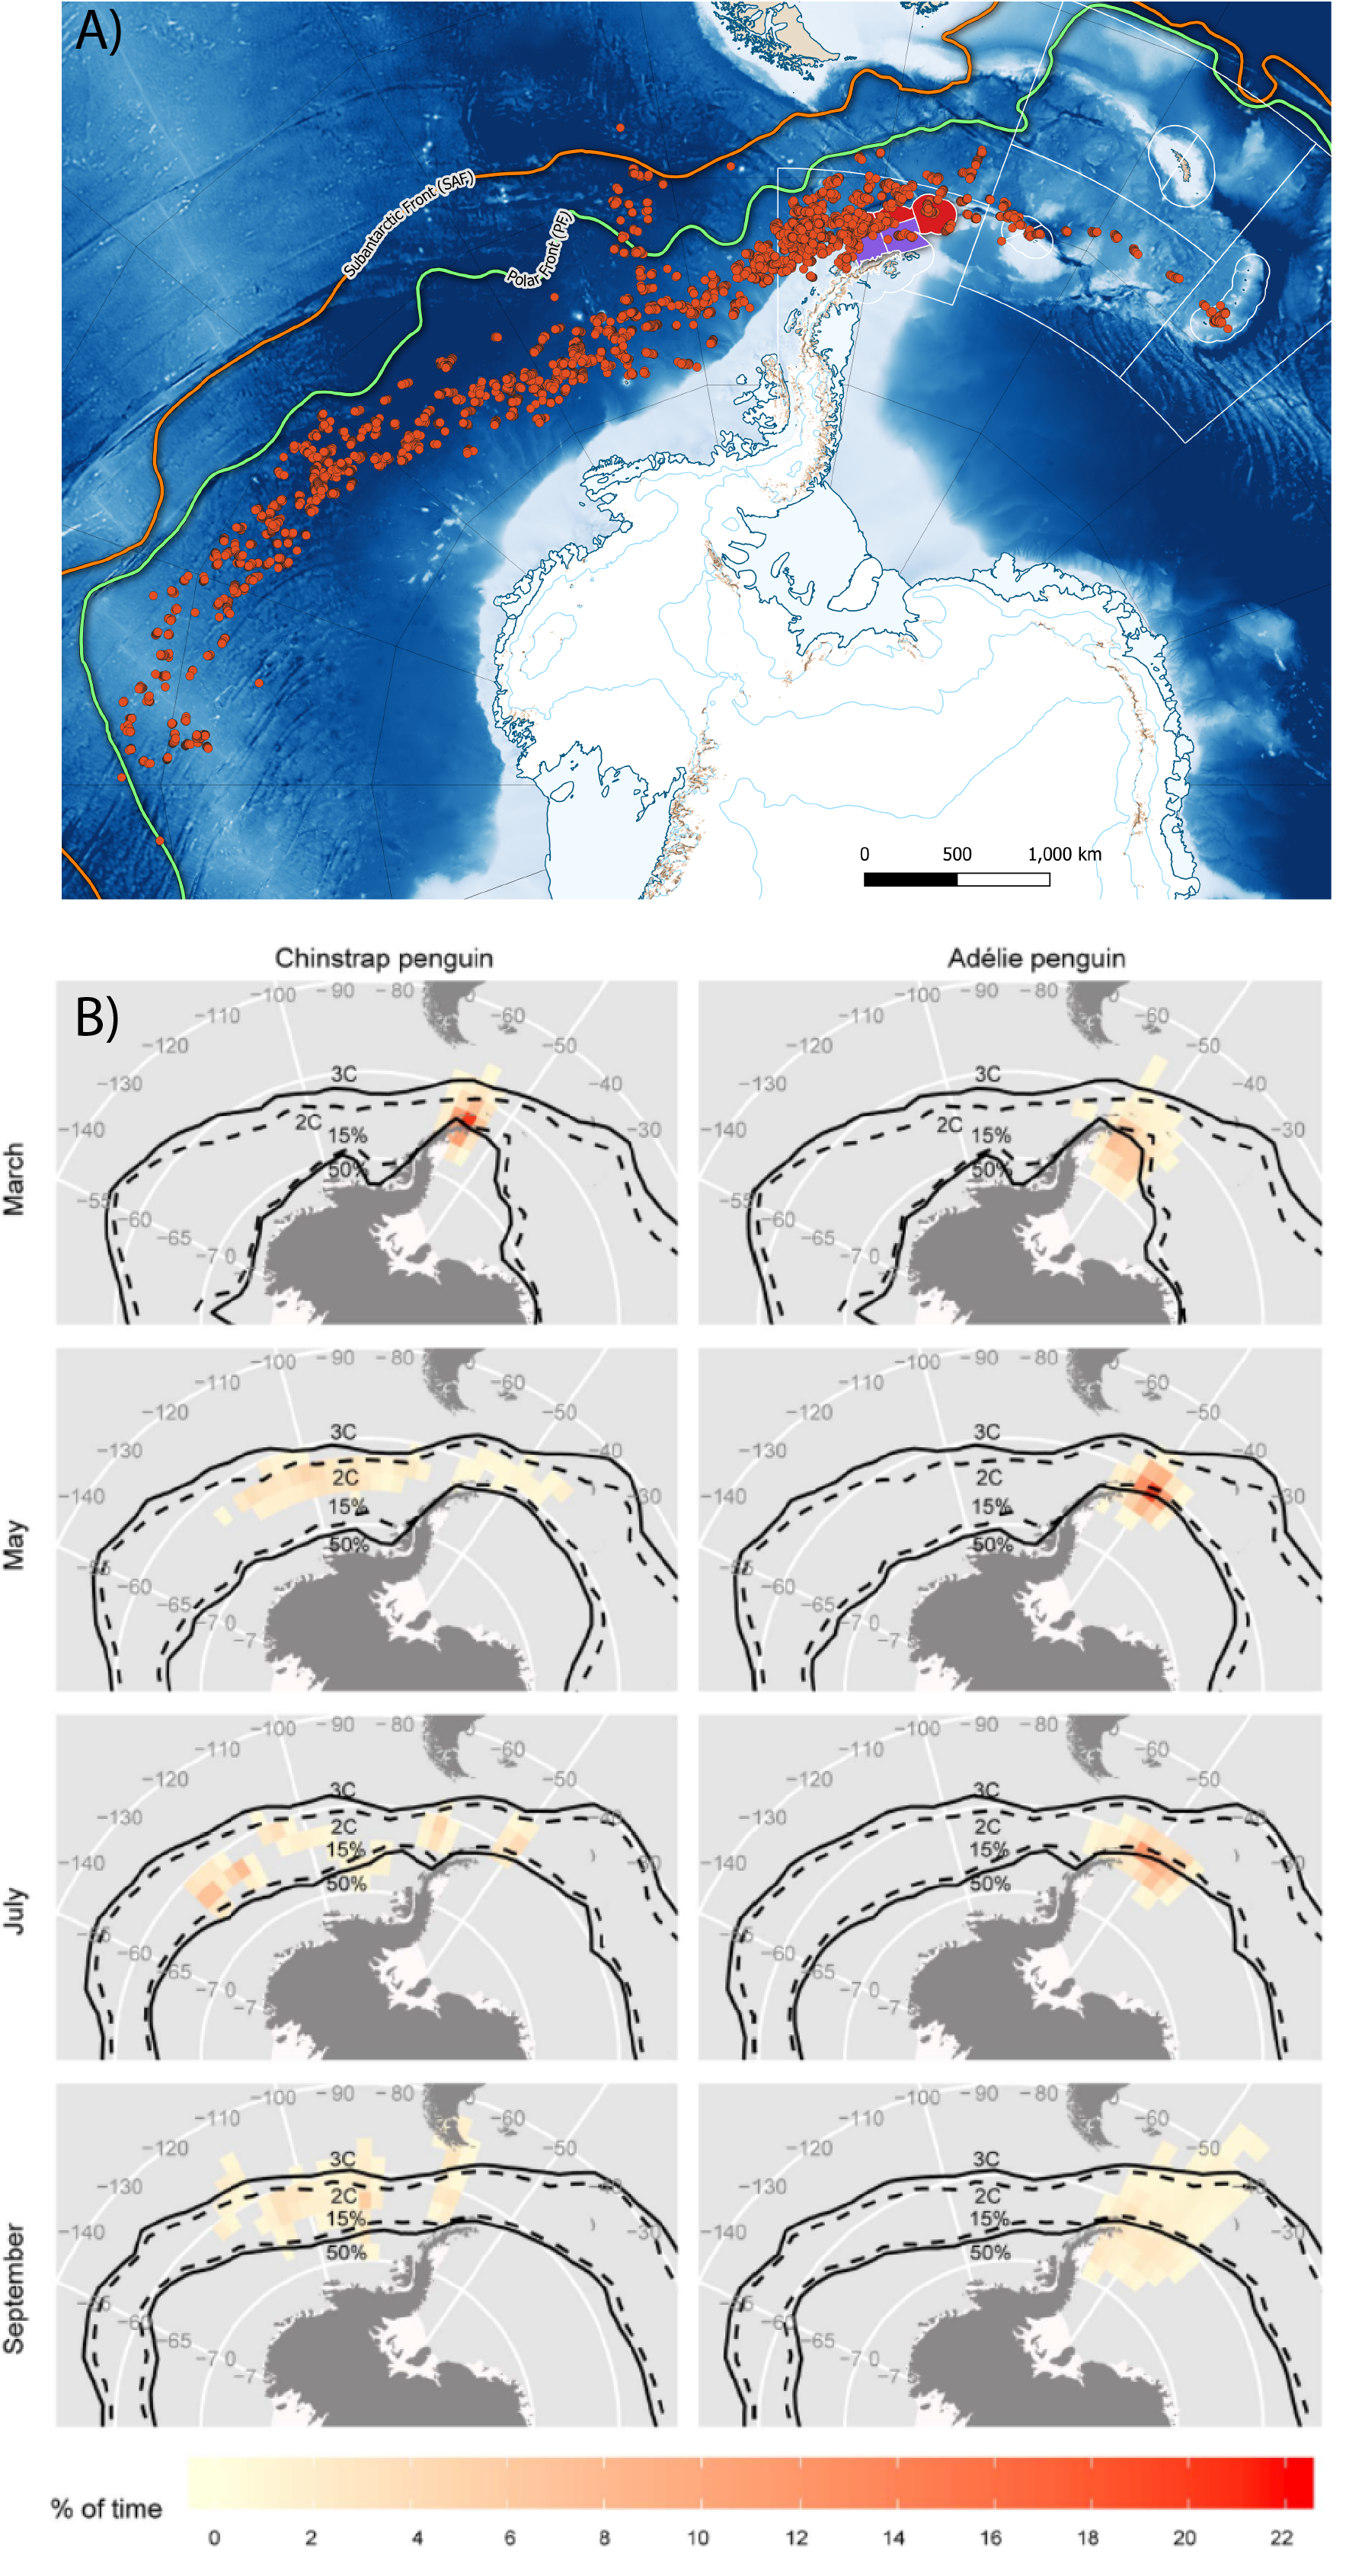
\includegraphics[width=0.75\linewidth]{C:/Users/Andy/Desktop/EMM paper figures/Watters EMM figures/Overwinter pengo distributions} \caption{A) Distribution of overwinter movement for Chinstrap penguins, relative to the gSSMU's to which they were attributed, created from telemetry data available in Hinke et al. 2019.  B) Adélie and Chinstrap penguin movement recorded by light geolocators, highlighting the large longitudinal range both species disperse through at the end of breeding (taken from Hinke et al. 2015).  In the original model formulation by Watters et al. 2020, the performance indices for both species are matched to gSSMU-scale estimates of LKB and LHR and macroscale levels of ONI variability.}\label{fig:Overwinter penguin distribution plots}
\end{figure}

\begin{figure}

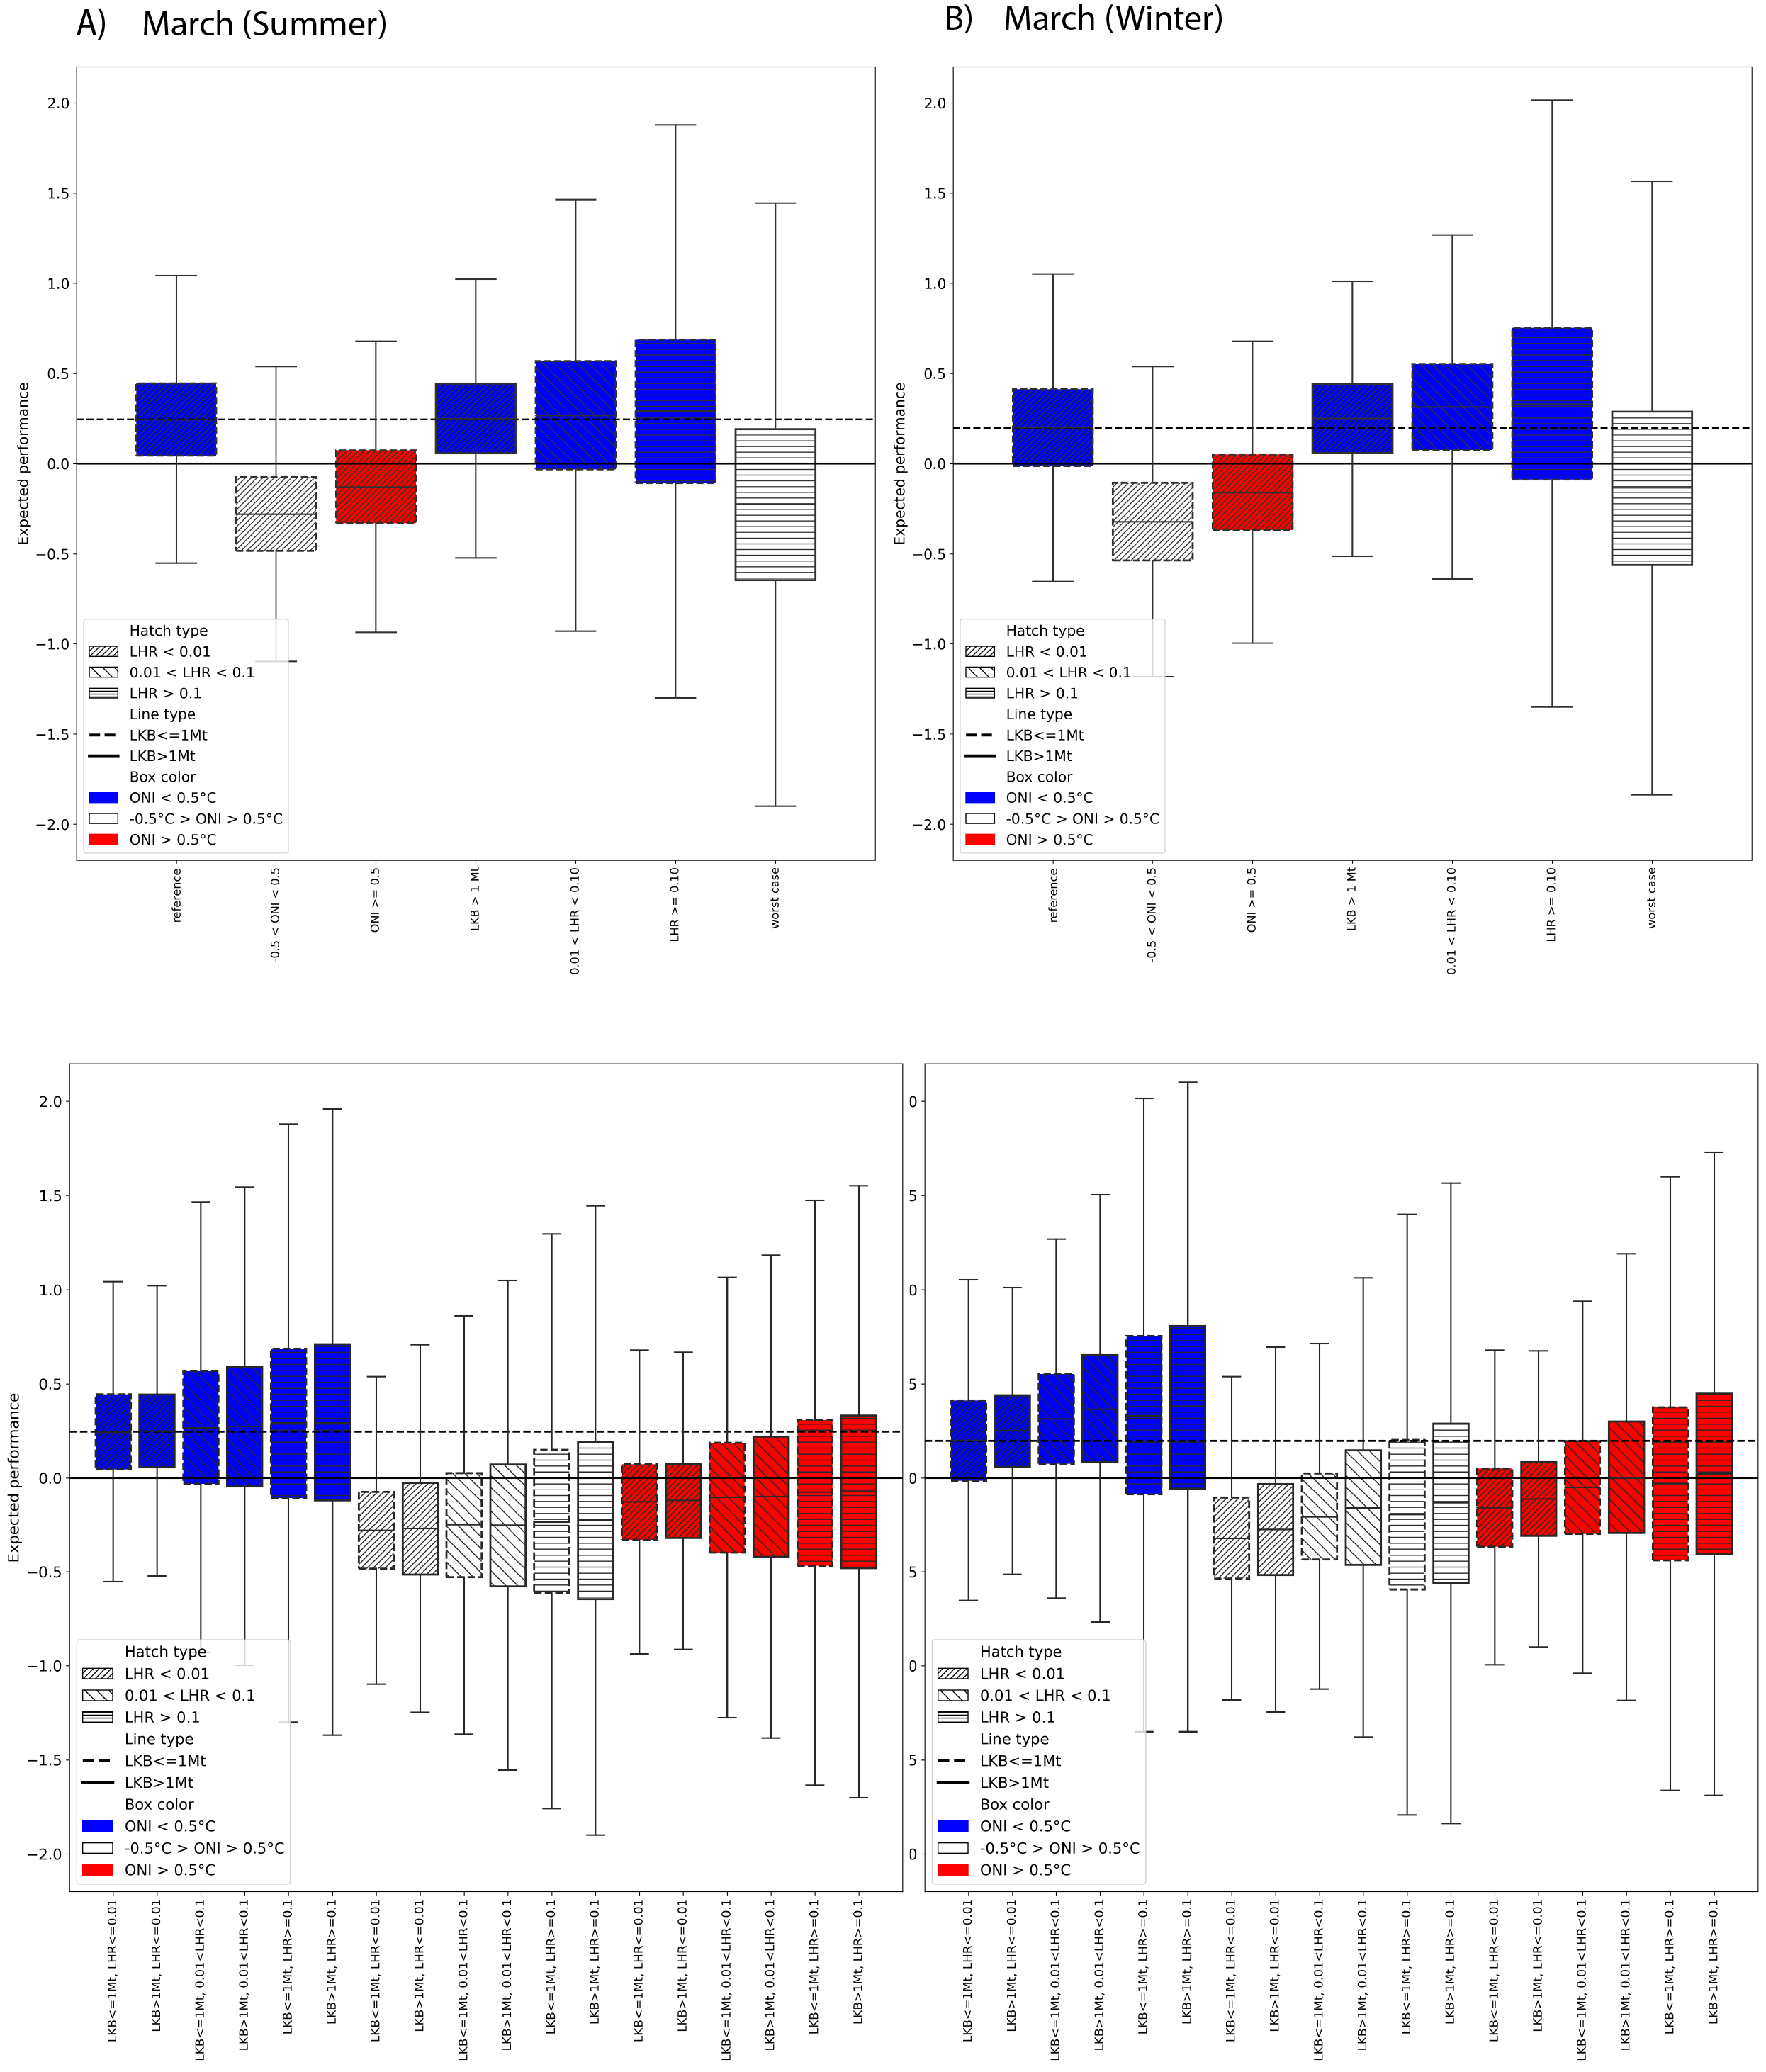
\includegraphics[width=1.3\linewidth]{C:/Users/Andy/Desktop/EMM paper figures/Watters EMM figures/All spp summer then winter 37} \hfill{}

\caption{Model output for Scenario \#1 outlined above (all species initially present,Adélie and Chinstrap penguins migrate out of the area after breeding, LKB and LHR rescaled to SSMU and March included in summer or winter).   Selected cases as per Watters et al. 2020 for March in A) Summer and B) Winter are provided, with the corresponding case-by-case boxplots presented beneath.  Boxplots are colour-coded by ONI state (red=warm, white=neutral, blue=cold).  In all cases, the marginal effect of ONI dominated the expected performance of penguins against their long-term mean, irrespective of LKB or LHR.}\label{fig:Scenario plot 1}
\end{figure}

\begin{figure}

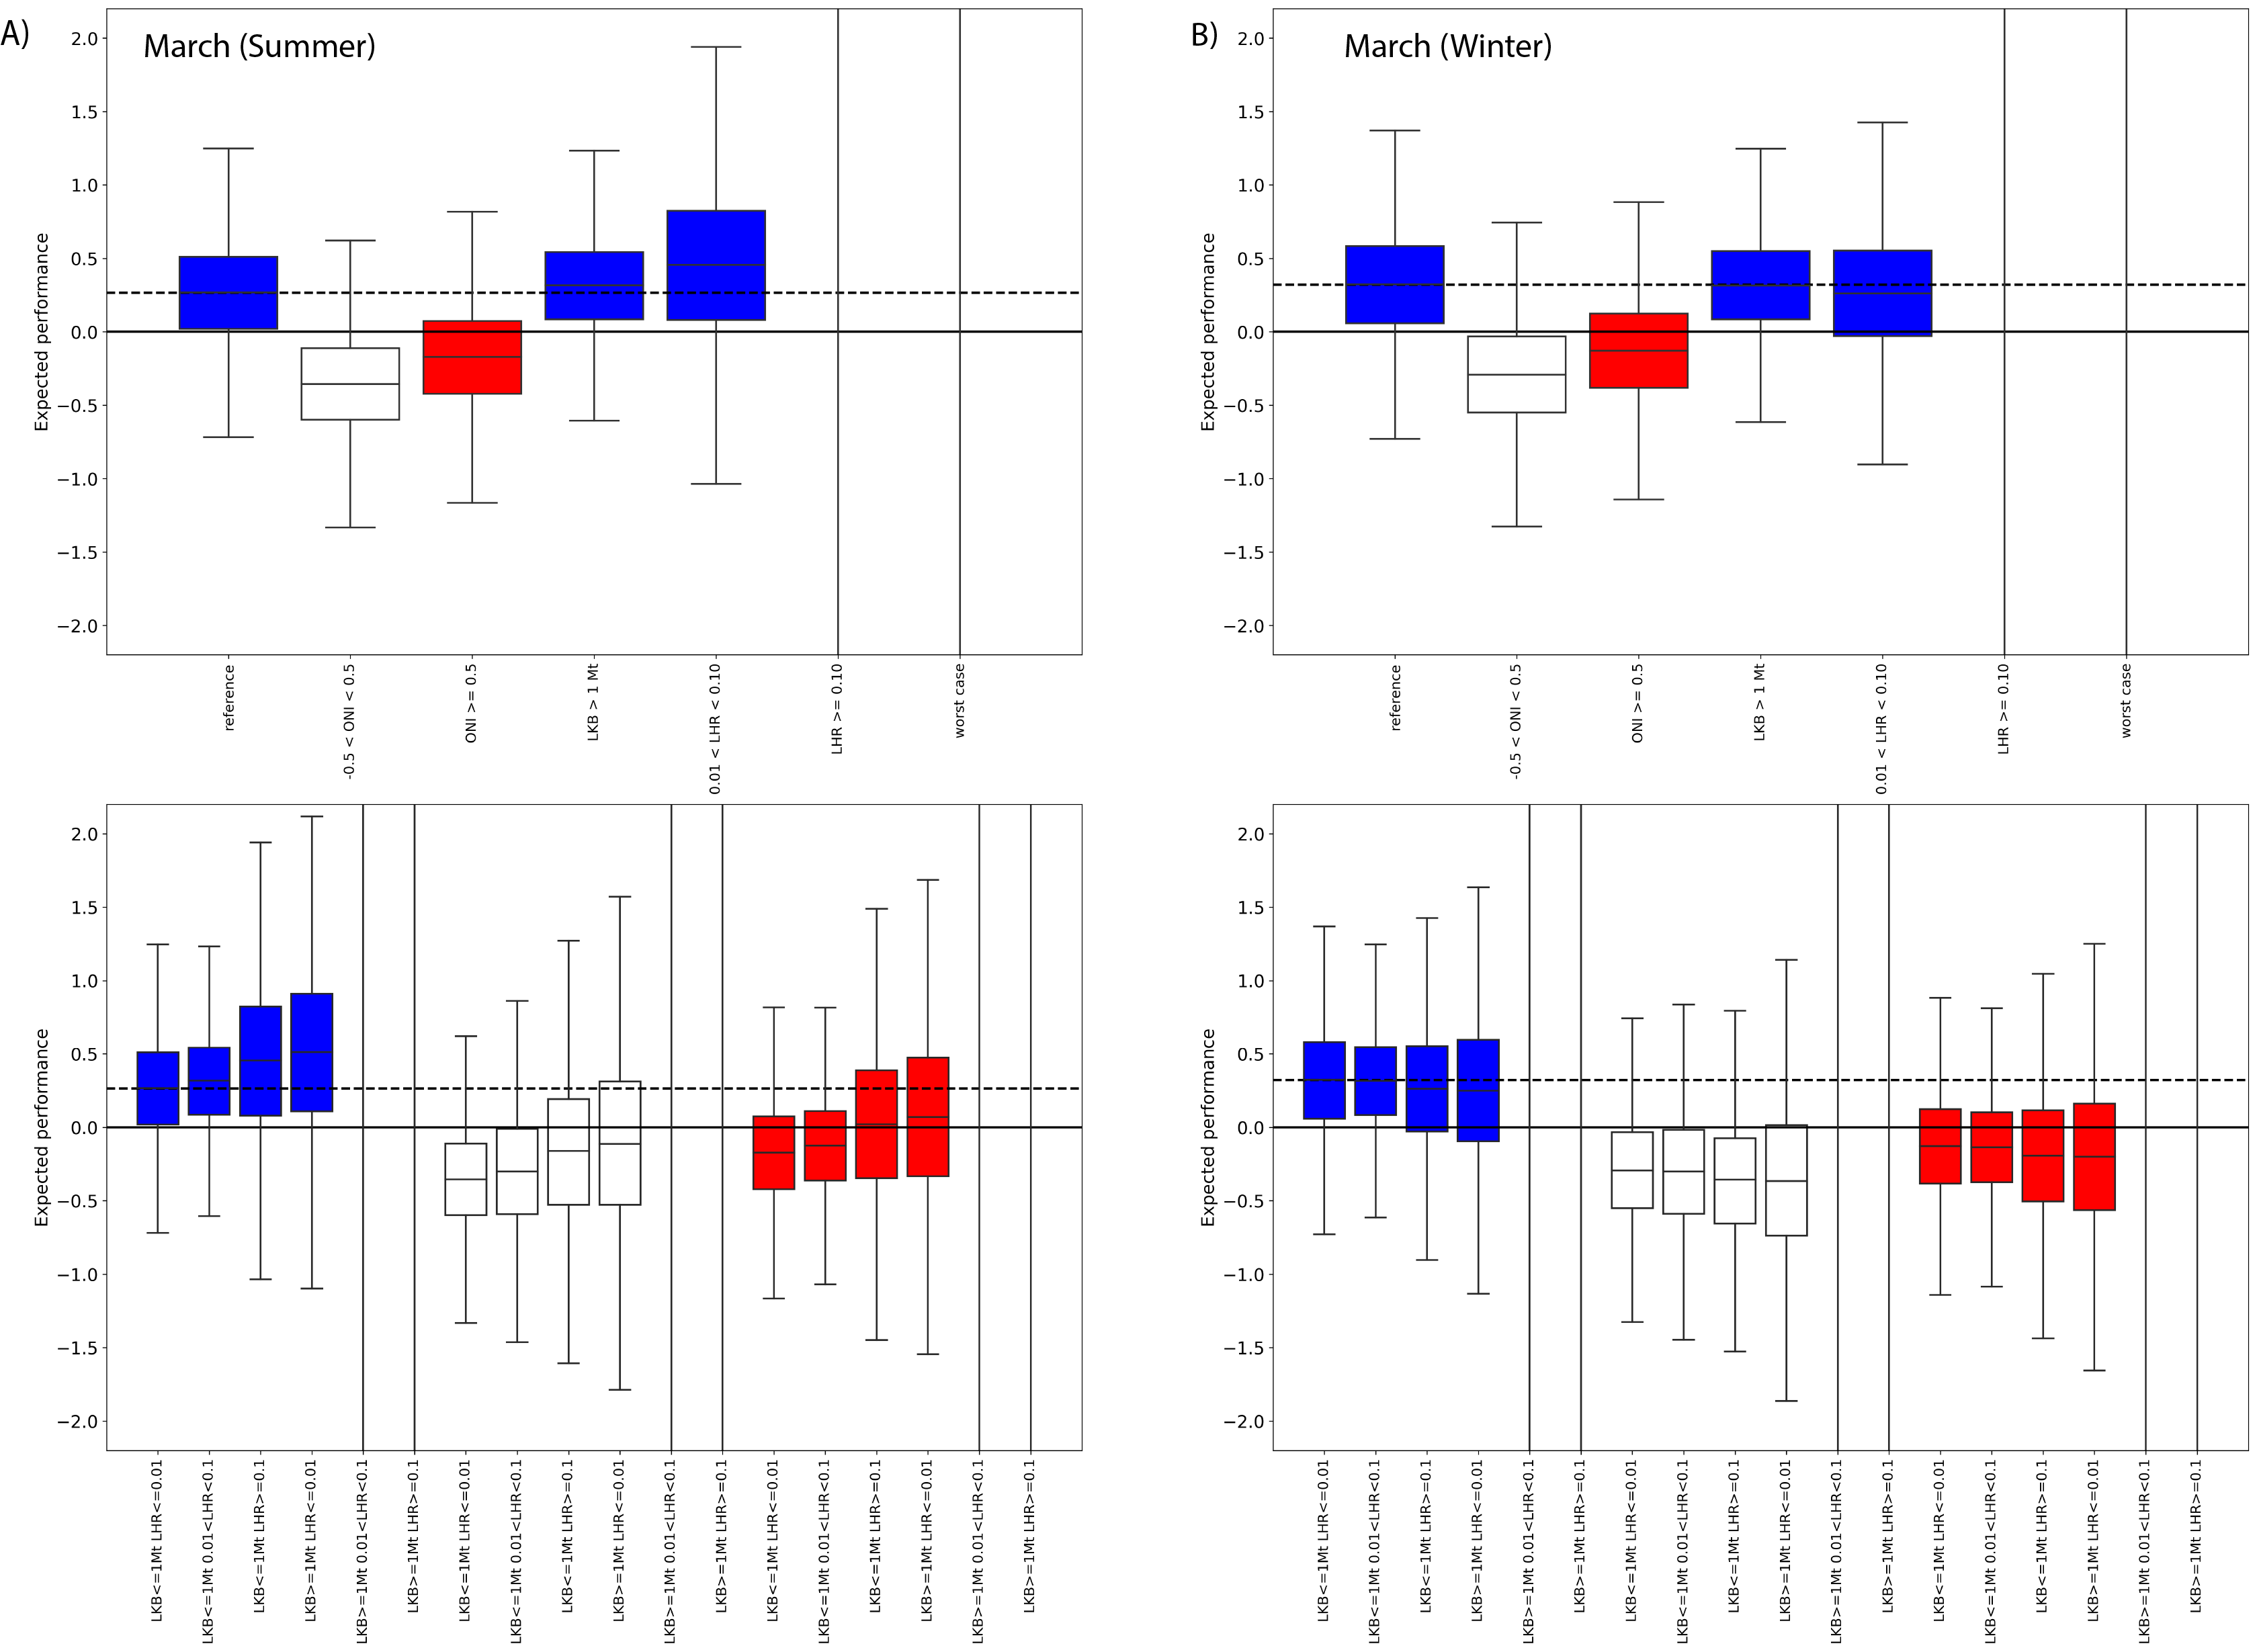
\includegraphics[width=1.3\linewidth]{C:/Users/Andy/Desktop/EMM paper figures/Watters EMM figures/ADE and CHIN summer 40 41} \hfill{}

\caption{Model output for Scenario \#2 outlined above (all species initially present,Adélie and Chinstrap penguins migrate out of the area after breeding, LKB and LHR rescaled to SSMU and March included in summer or winter).   Selected cases as per Watters et al. 2020 for March in A) Summer and B) Winter are provided, with the corresponding case-by-case boxplots presented beneath.  Boxplots are colour-coded by ONI state (red;warm, white;neutral, blue;cold).  In all cases, the marginal effect of ONI dominated the expected performance of penguins against their long-term mean, irrespective of LKB or LHR.}\label{fig:Scenario plot 2}
\end{figure}

\begin{figure}

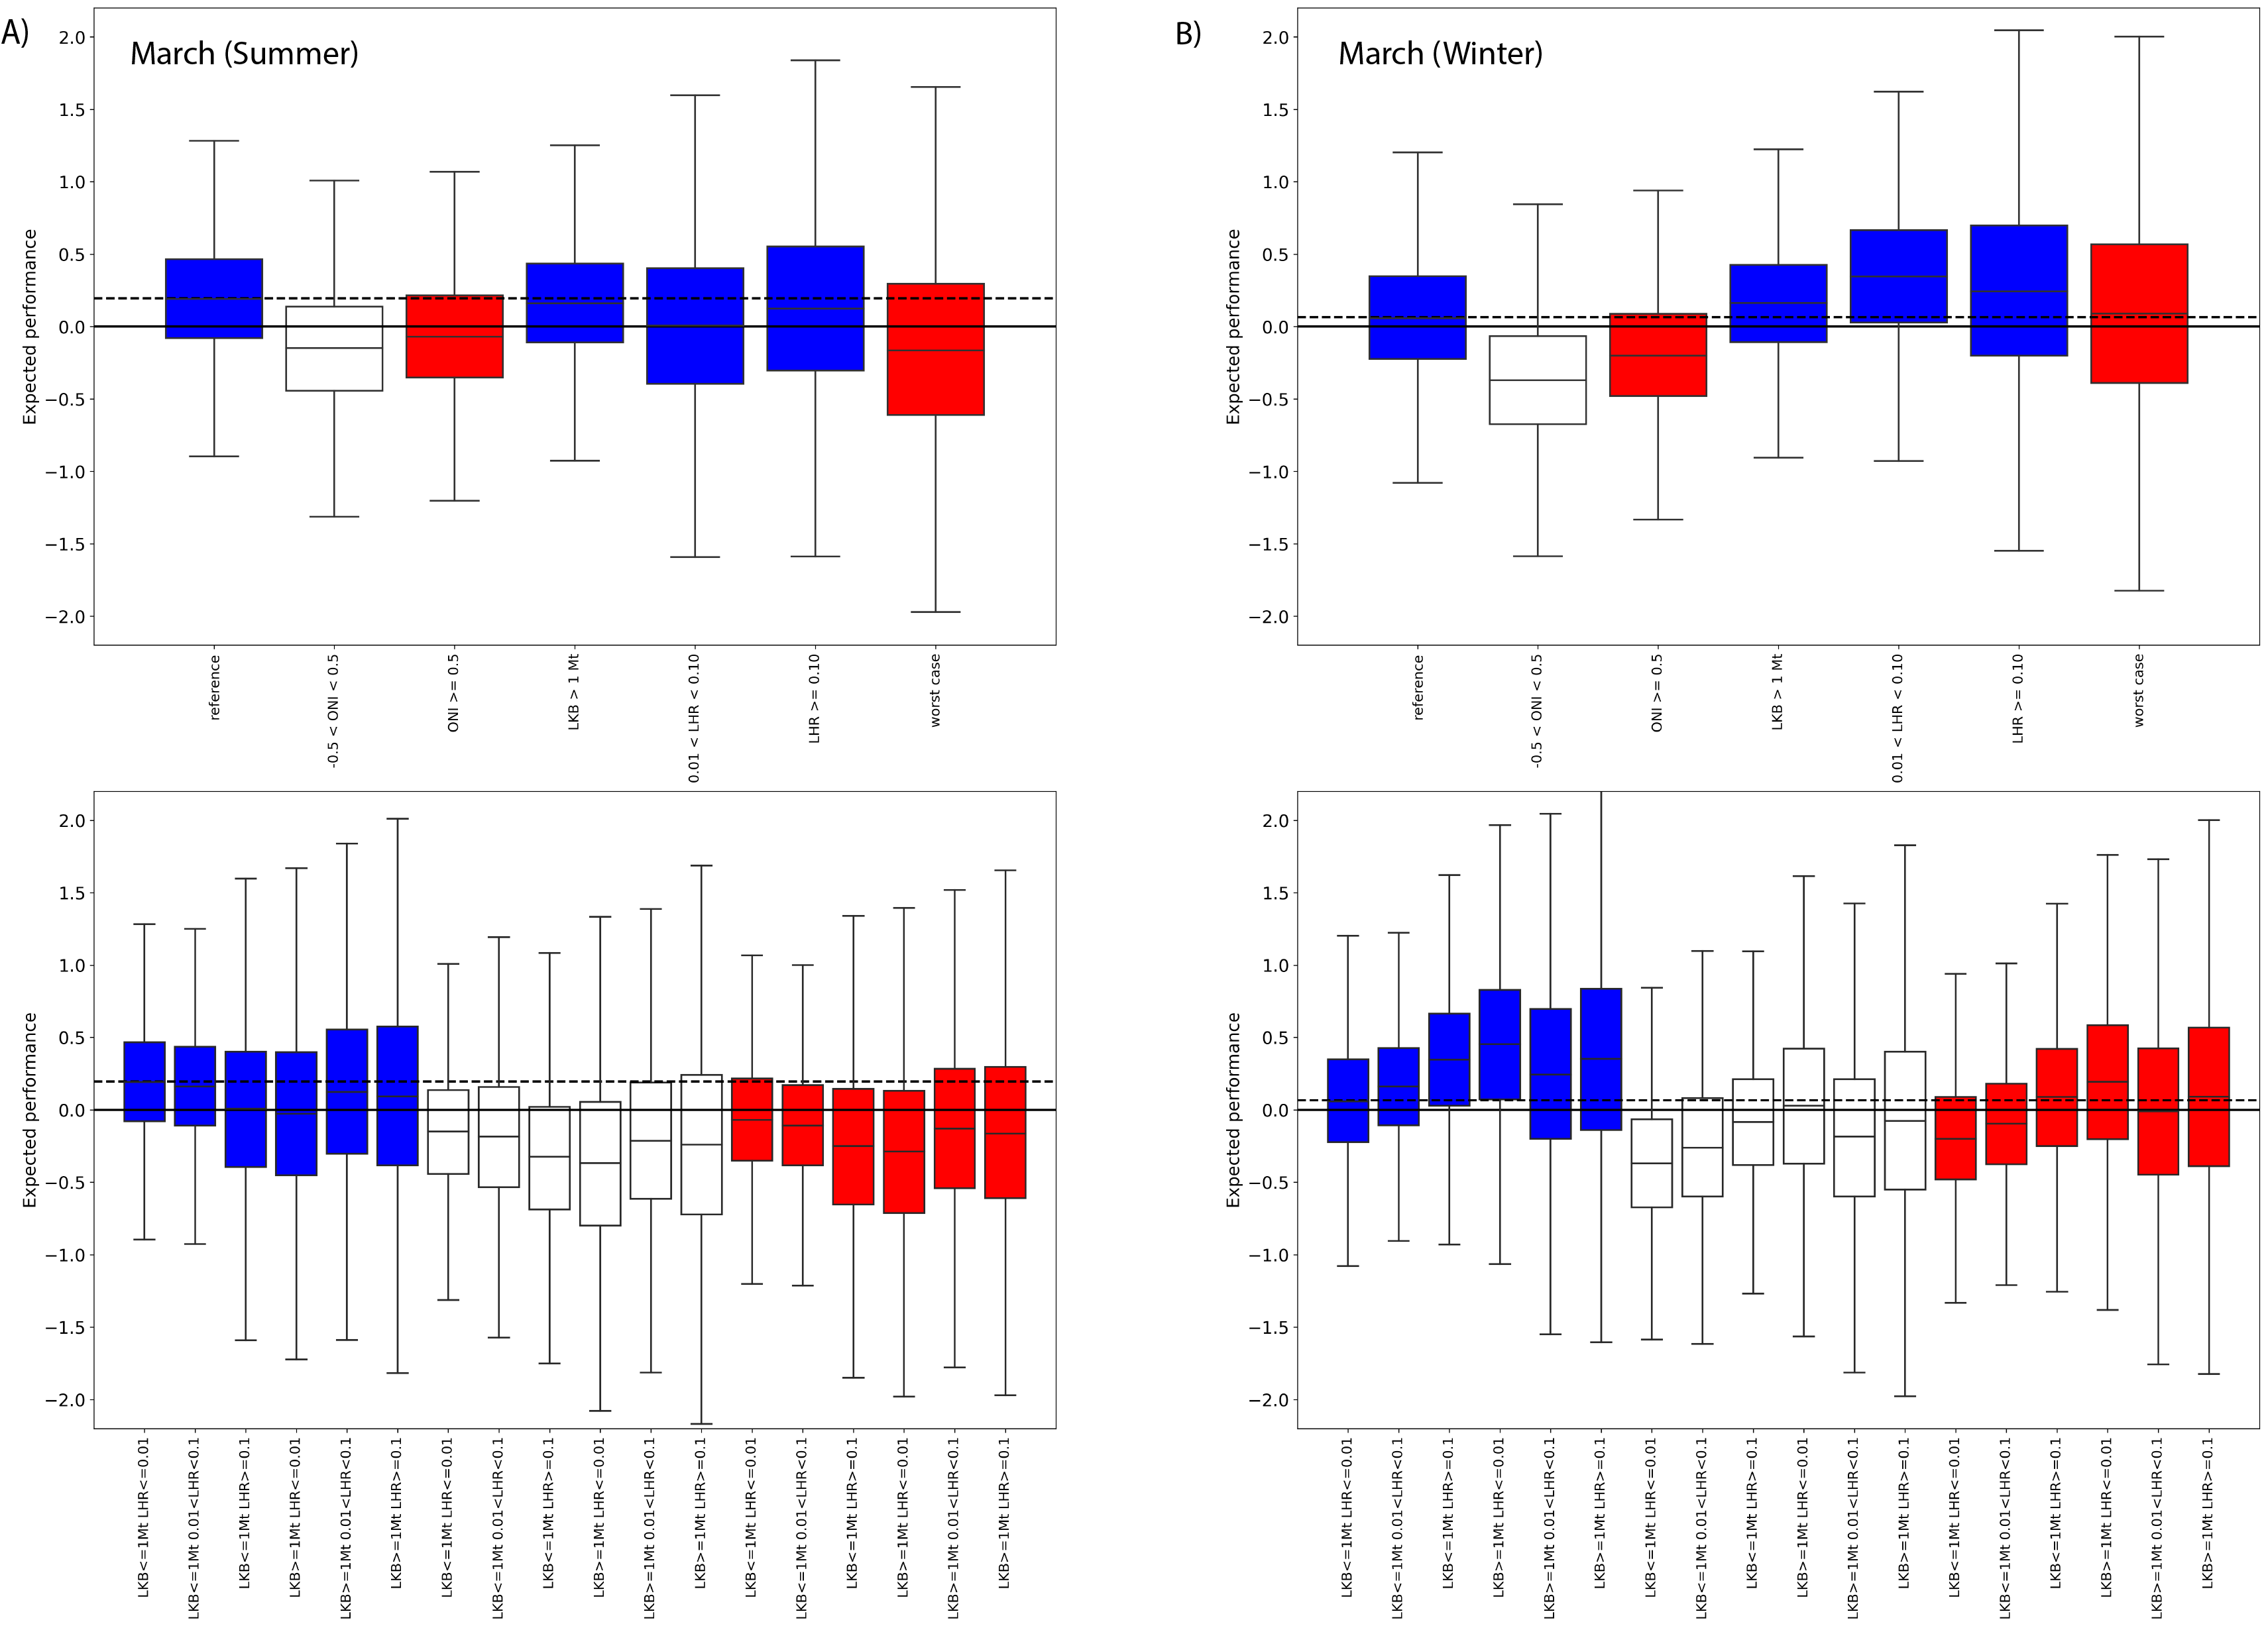
\includegraphics[width=1.3\linewidth]{C:/Users/Andy/Desktop/EMM paper figures/Watters EMM figures/Gentoo only 38 39} \hfill{}

\caption{Model output for Scenario \#3 outlined above (all species initially present,Adélie and Chinstrap penguins migrate out of the area after breeding, LKB and LHR rescaled to SSMU and March included in summer or winter).   Selected cases as per Watters et al. 2020 for March in A) Summer and B) Winter are provided, with the corresponding case-by-case boxplots presented beneath.  Boxplots are colour-coded by ONI state (red;warm, white;neutral, blue;cold).  In all cases, the marginal effect of ONI dominated the expected performance of penguins against their long-term mean, irrespective of LKB or LHR.}\label{fig:Scenario plot 3}
\end{figure}

\begin{figure}
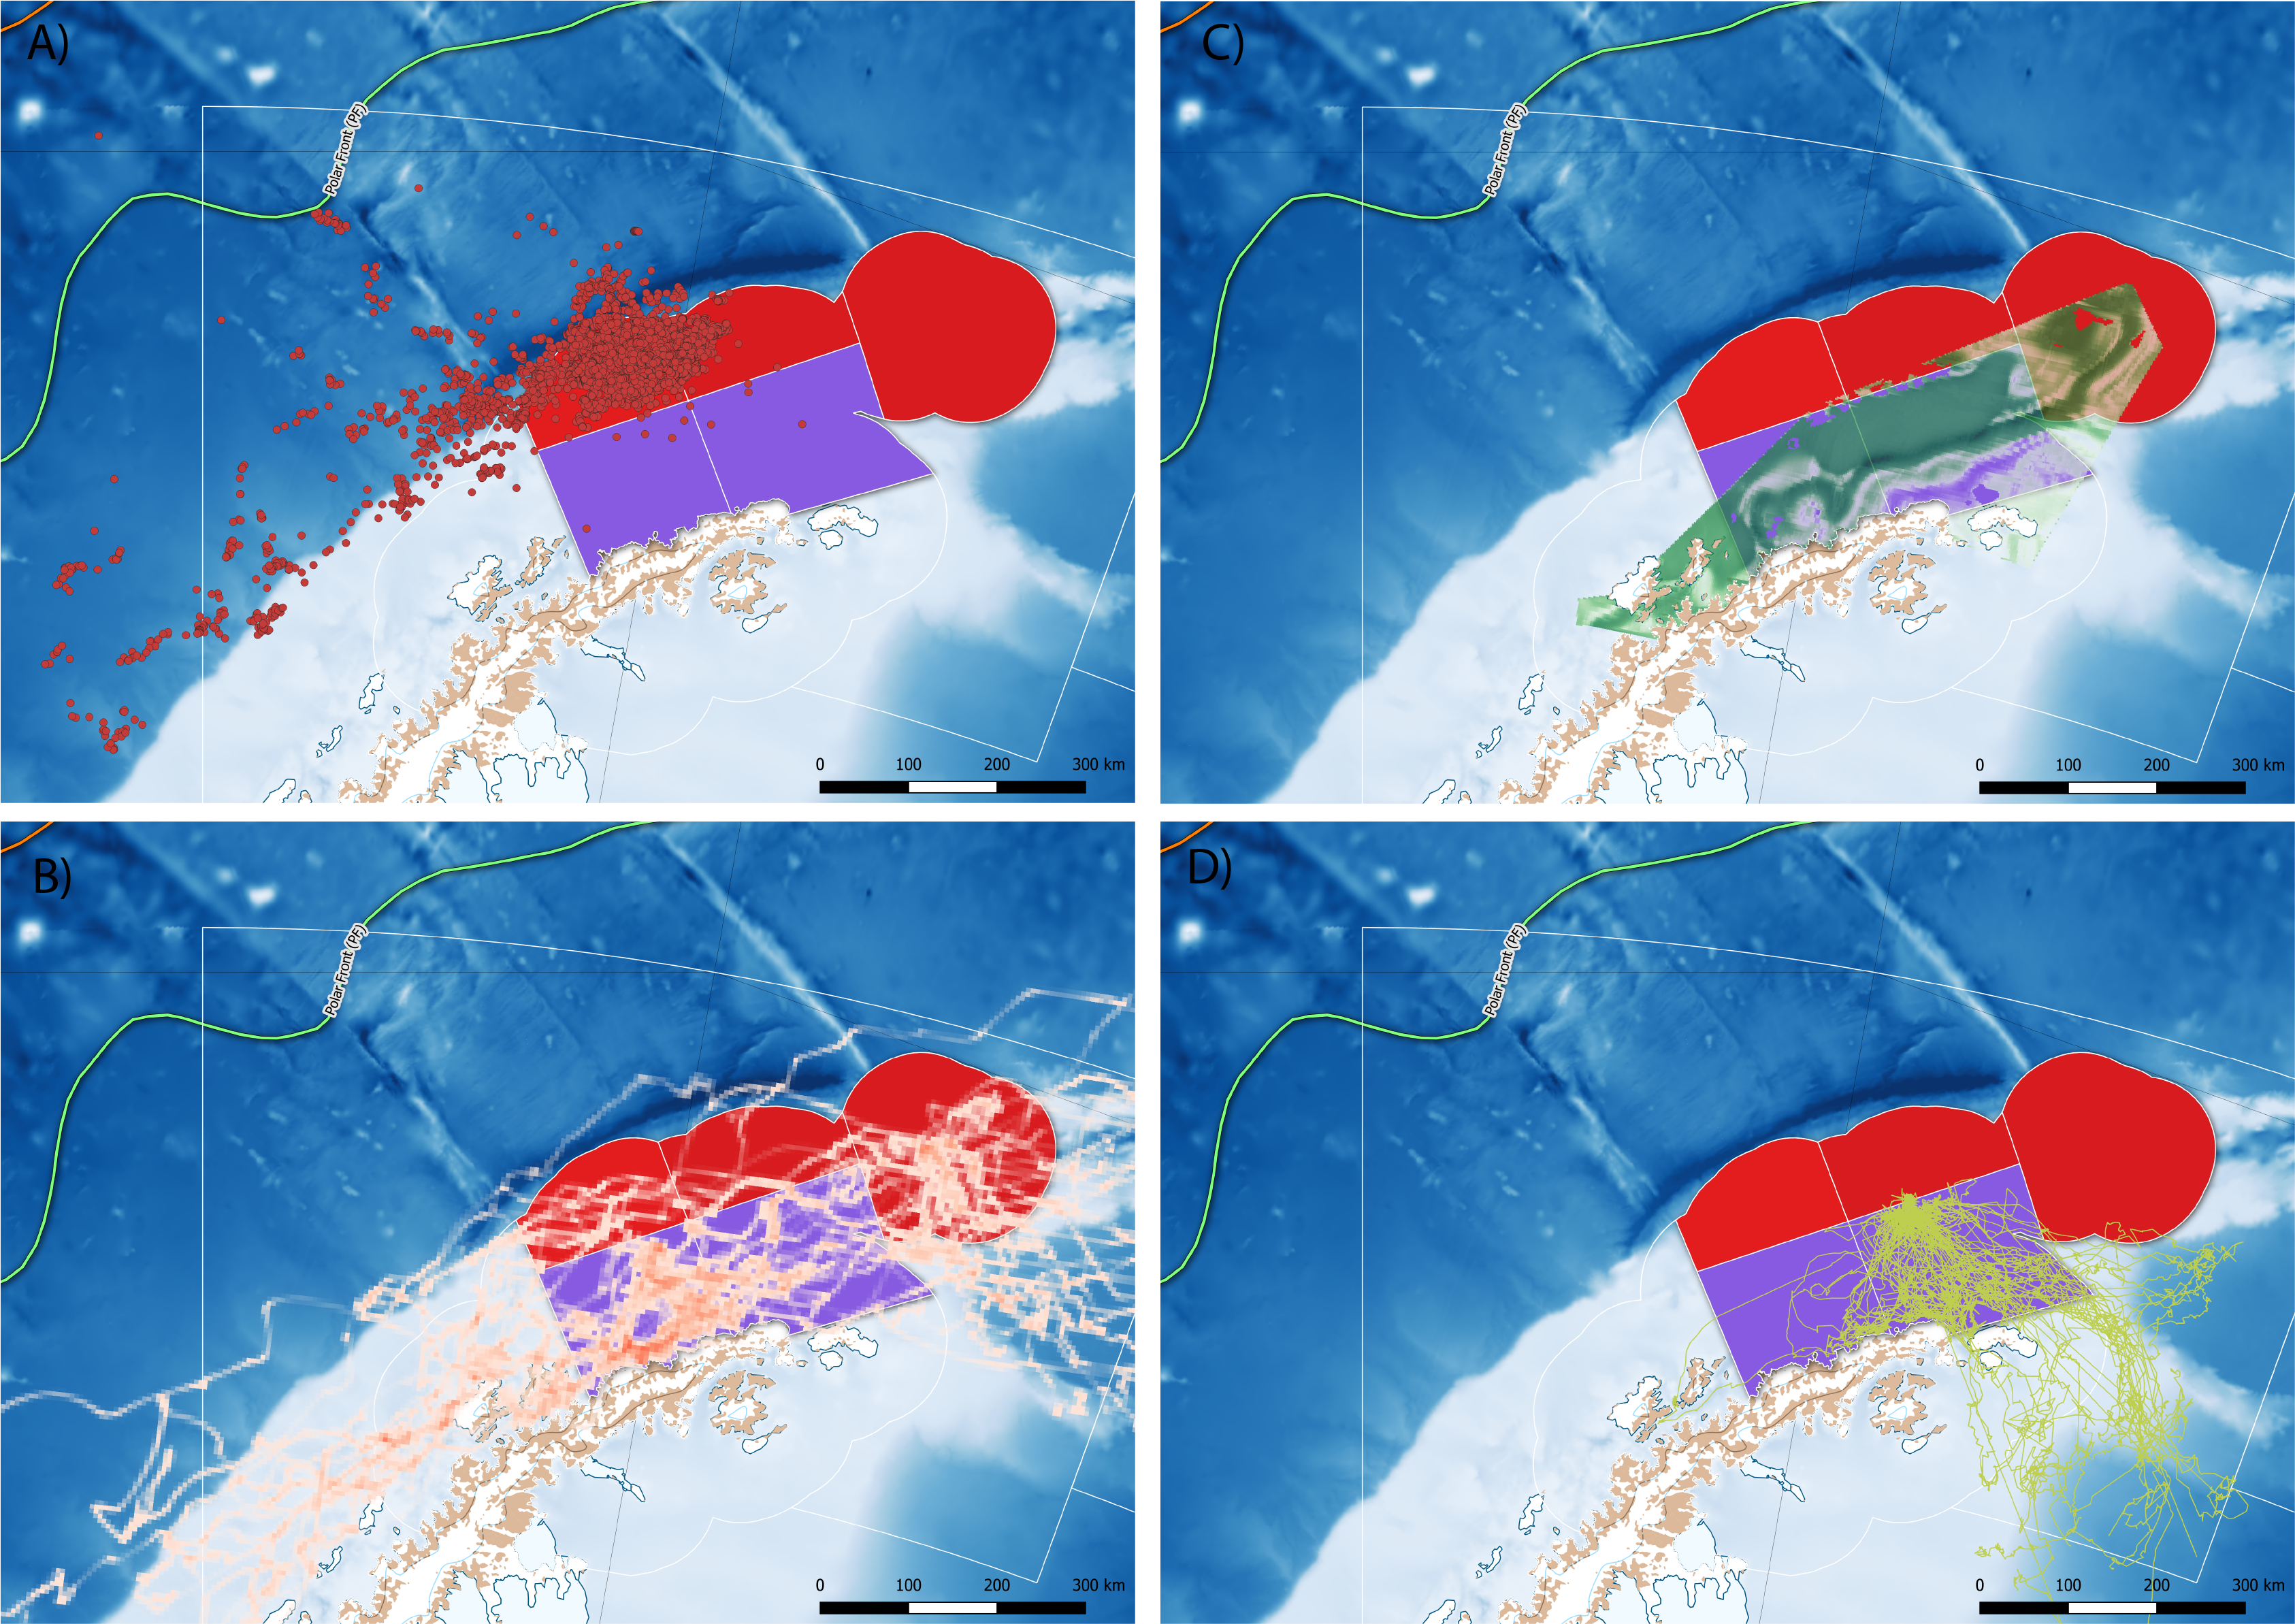
\includegraphics[width=1.2\linewidth]{C:/Users/Andy/Desktop/EMM paper figures/Watters EMM figures/Other spp distribution} \caption{The summer distribution of foraging effort by A) adult female Antarctic fur seals (adapted from telemetry data available in Hinke et al. 2017), B) migratory adult male Antarctic fur seals (adapted from Lowther et al. 2020) C) humpback whales throughout December (adapted from Johannessen et al., this meeting) and D) nonbreeding adult Adélie penguins during the breeding season (adapted from data in Oosthuizen et al., this meeting). Potential effects of competitive overlap between pygoscelid penguins and other krill dependent predators, particularly those who have increased their abundance dramatically over the preceding 40 years, are excluded from both approaches, creating an unrealistic set of boundary conditions for interpreting the variance in penguin vital rates.}\label{fig:other species plots}
\end{figure}

\begin{figure}
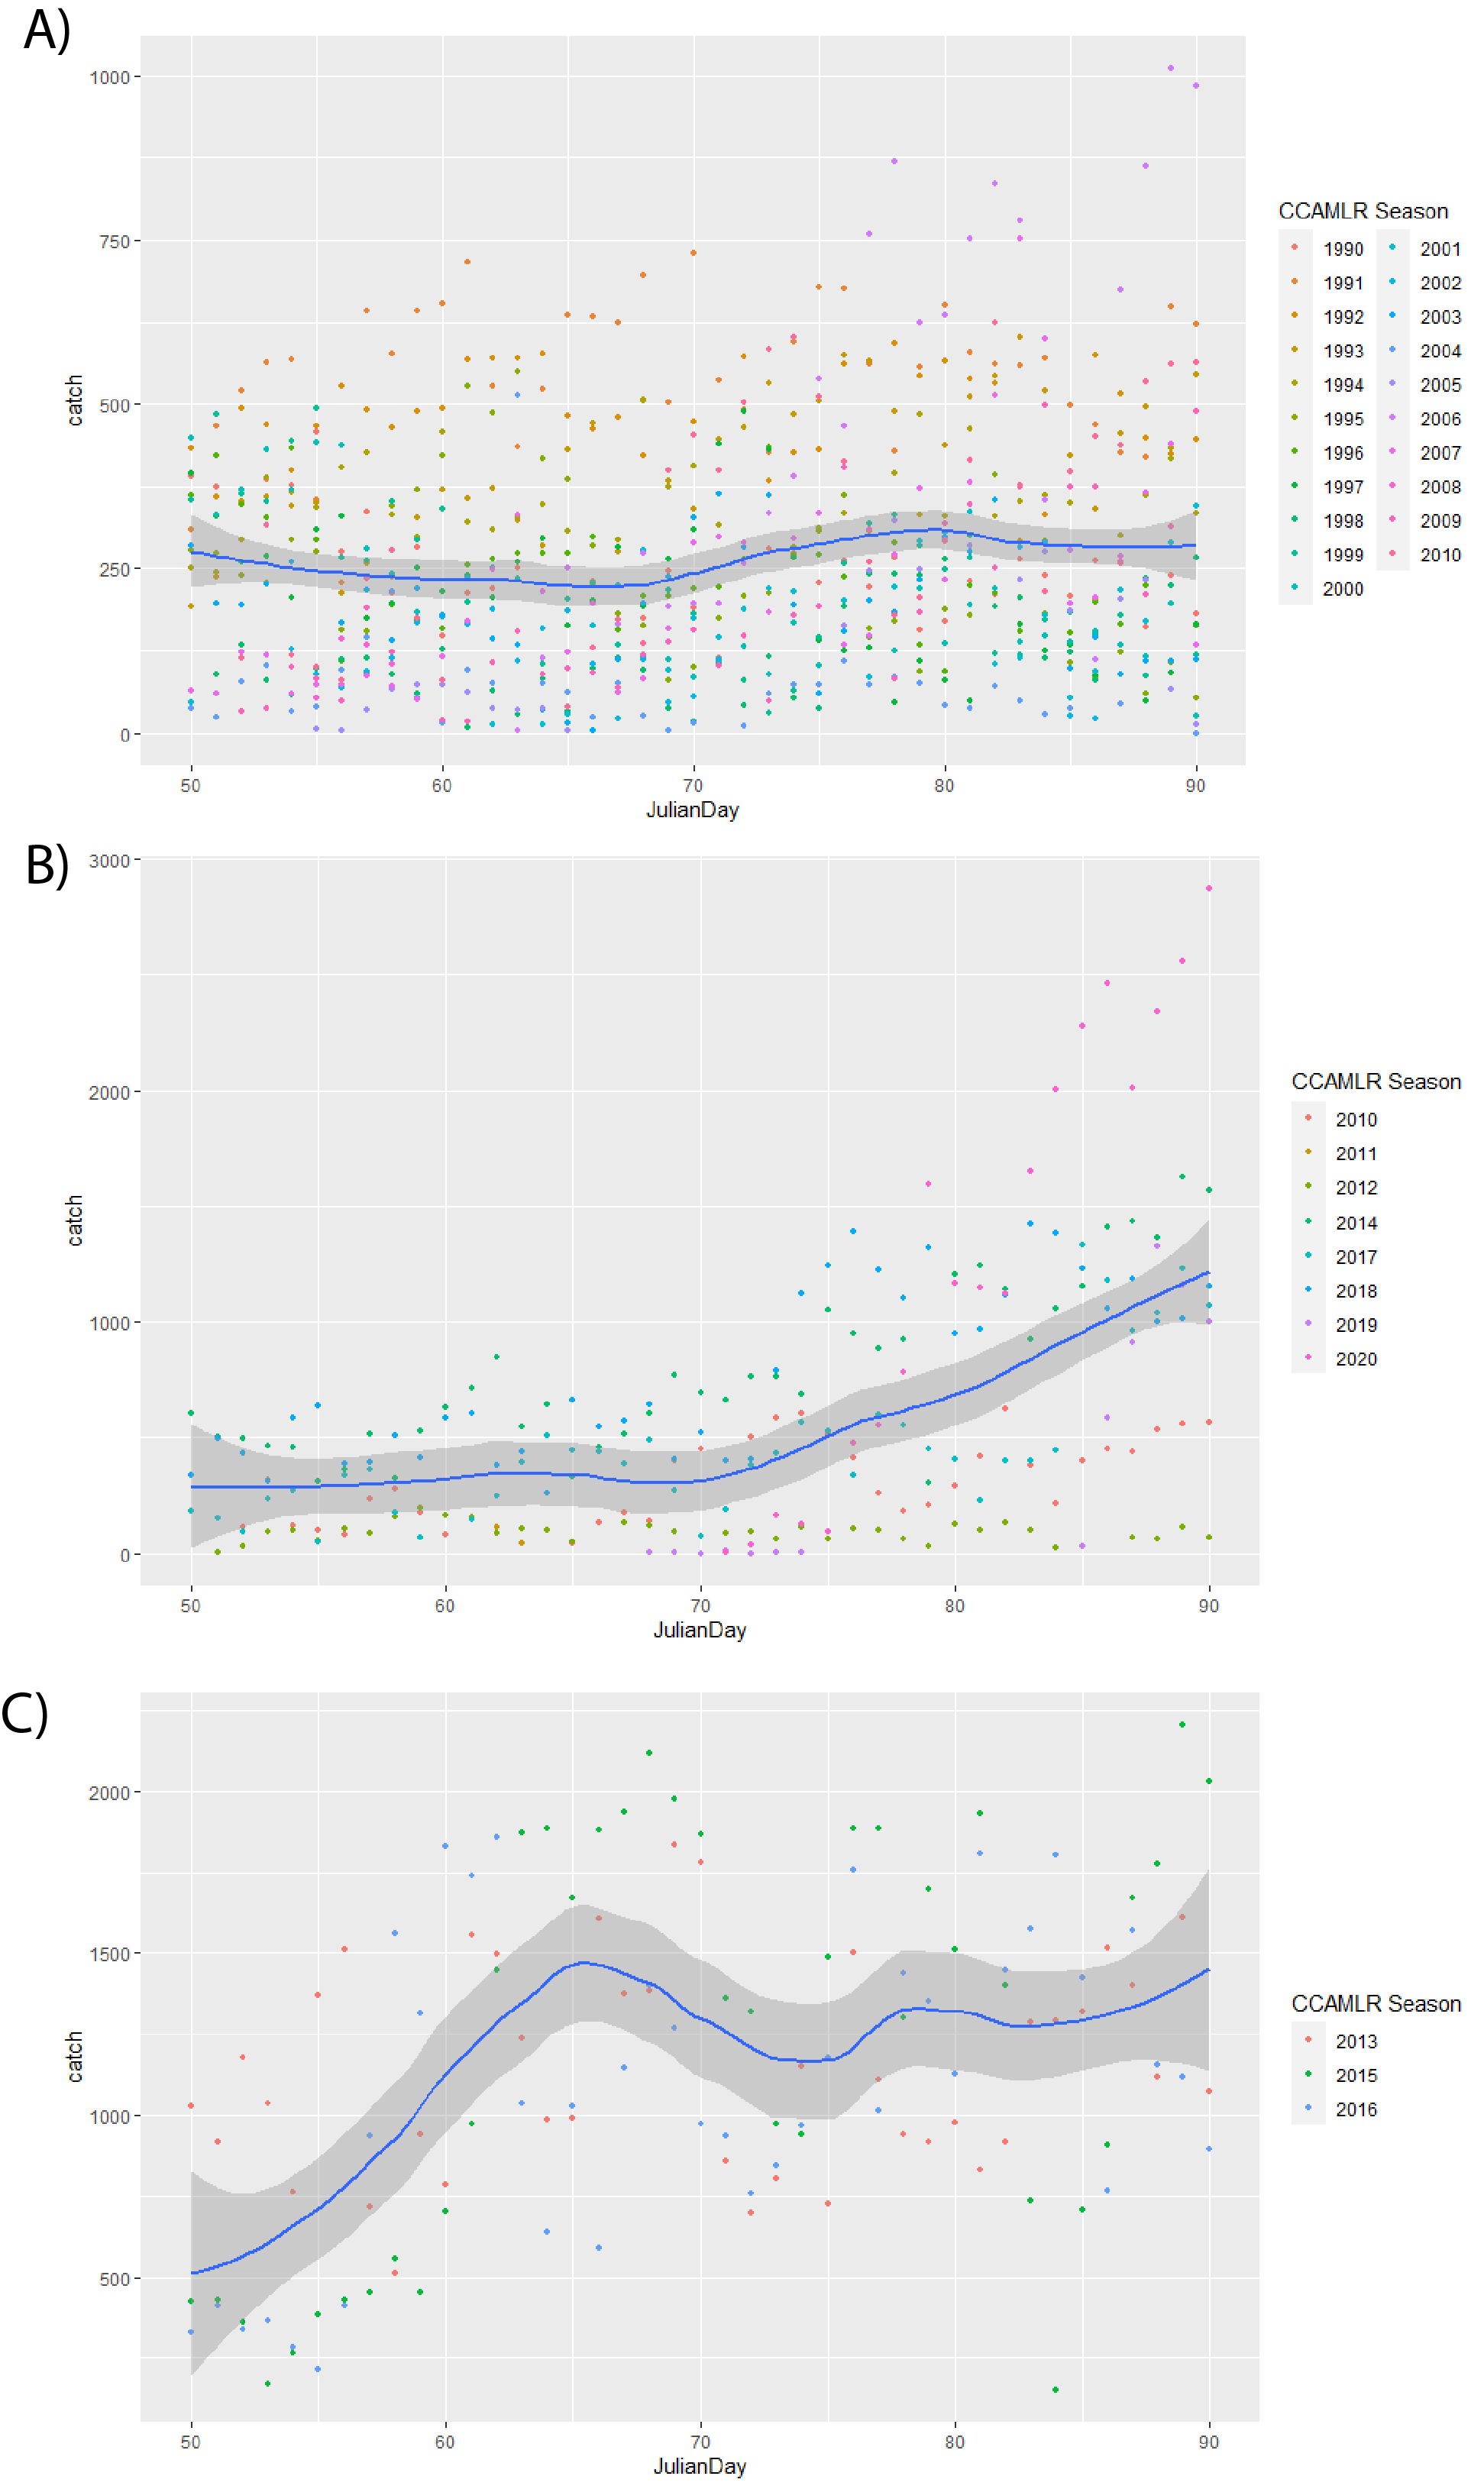
\includegraphics[width=0.9\linewidth]{C:/Users/Andy/Desktop/EMM paper figures/Watters EMM figures/48.1 catches in march} \caption{Daily accumulated catch (and fitted LOESS smooth curves) in Subarea 48.1 between 20$^{th}$ February and March 31$^{st}$ between A) 1990-2010 and B) 2010 to 2020. Catch in the Subarea was relatively consistent during the latter stages of penguin breeding at approximately 250tonnes/d.  However, since 2010 there has been a tendency for the fishery to increase its effort in the Subarea, starting around the middle of March. C) During this latter period, the fishery increased effort earlier on three occasions (2013, 2015 and 2016), starting before the beginning of March.}\label{fig:March Subarea 48.1 fishing plot}
\end{figure}


\end{document}


